\documentclass[sigconf,nonacm]{acmart}

% Packages
\usepackage{graphicx}
\usepackage{booktabs}
\usepackage{algorithm}
\usepackage{algpseudocode}
\usepackage{tikz}
\usetikzlibrary{positioning,shapes.geometric,arrows.meta,fit,calc,patterns,shapes.misc,decorations.pathreplacing}
\usepackage{pgfplots}
\pgfplotsset{compat=1.18}
\usepackage{subcaption}
\usepackage{float}
\usepackage{hyperref}

% Custom commands
\newcommand{\agg}{\mathrm{AGG}}
\newcommand{\concat}{\mathrm{CONCAT}}
\newcommand{\relu}{\mathrm{ReLU}}

% Remove ACM copyright/conference info
\settopmatter{printacmref=false}
\renewcommand\footnotetextcopyrightpermission[1]{}
\pagestyle{plain}

% Bibliography file
\citestyle{acmauthoryear}

% Document metadata
\title{Applying GraphSAGE to Large-Scale Node Classification}
\subtitle{Programming Machine Learning Algorithms for HPC - Final Report}

\author{Thomas Gantz}
\affiliation{%
  \institution{University of Luxembourg}
  \country{Luxembourg}
}
\email{thomas.gantz.001@student.uni.lu}

\author{Alberto Finardi}
\affiliation{%
  \institution{University of Luxembourg}
  \country{Luxembourg}
}
\email{alberto.finardi.001@student.uni.lu}

\author{Tommaso Crippa}
\affiliation{%
  \institution{University of Luxembourg}
  \country{Luxembourg}
}
\email{tommaso.crippa.001@student.uni.lu}

\author{Jan Esquivel Marxen}
\affiliation{%
  \institution{University of Luxembourg}
  \country{Luxembourg}
}
\email{jan.esquivel.001@student.uni.lu}

\begin{document}

\begin{abstract}
This report documents our study and application of GraphSAGE (Graph SAmple and aggreGatE)~\cite{graphsage}, an inductive framework for learning node embeddings on large-scale graphs. We provide background on graph neural networks and the message passing paradigm, then describe how GraphSAGE addresses the scalability limitations of earlier approaches by learning aggregator functions rather than fixed node embeddings. We apply GraphSAGE to the ogbn-products benchmark dataset for node classification, detailing our implementation choices, hyperparameter tuning process, and experimental results.\\[0.2cm]
\textit{Code and experiments available at: \url{https://github.com/albertofinardi/Sage_GNN}}
\end{abstract}

\maketitle

%=======================================================================
\section{Introduction}
\label{sec:introduction}
%=======================================================================

Graph-structured data appears in many domains, including social networks, citation graphs, biological networks, and recommendation systems. A central challenge is learning node representations (embeddings) that capture both node features and structural context.

\paragraph{Graph Prediction Tasks.}
Machine learning on graphs encompasses node-level prediction (classifying individual nodes), edge-level prediction (link prediction or edge classification), and graph-level prediction (predicting properties of entire graphs). This report focuses on \textbf{node classification}, One of the possible applications of GraphSAGE.

\paragraph{Graph Neural Networks.}
A Graph Neural Network (GNN) is a learnable transformation that updates node features using neural networks, respects graph structure by aggregating neighbor information, and is permutation invariant. GNNs build node representations through iterative \textbf{message passing}: at each layer, nodes gather neighbor embeddings, aggregate them with a permutation-invariant function, and apply a learned transformation.

\paragraph{Limitations of Prior Methods.}
Before GraphSAGE, methods like DeepWalk and node2vec~\cite{deepwalk,node2vec} learned embeddings via random walks but were \textit{transductive} - adding new nodes required retraining. GCNs~\cite{gcn} use message passing but operate on the full adjacency matrix, limiting scalability. The fundamental problem: \textbf{no method provided a parametric function to generate embeddings for unseen nodes.}

\paragraph{The GraphSAGE Insight.}
GraphSAGE's innovation is to learn a \textbf{function} that generates embeddings rather than learning fixed embeddings per node. By learning aggregator functions that sample and combine neighborhood features, GraphSAGE becomes \textbf{inductive}: the model generalizes to new nodes or graphs without retraining.

%=======================================================================
\section{GraphSAGE Framework}
\label{sec:graphsage-framework}
%=======================================================================

GraphSAGE (Graph SAmple and aggreGatE) implements inductive learning through neighbor sampling and learned aggregation. At each layer $k$, node $v$ updates its representation by sampling neighbors, aggregating their embeddings, concatenating with its own embedding, and applying a learned transformation with non-linearity.

\subsection{Neighbor Sampling}
\label{subsec:sampling}

For scalability, GraphSAGE uniformly samples a fixed-size set of neighbors at each layer rather than using all neighbors. For a $K$-layer model with sample sizes $S_1, \ldots, S_K$, per-node complexity is $O(\prod_{k=1}^{K} S_k)$, independent of actual node degrees.

\subsection{Aggregator Functions}
\label{subsec:aggregators}

GraphSAGE supports several aggregators: \textbf{mean} (element-wise average of neighbor embeddings), \textbf{LSTM} (applies an LSTM network to aggregate neighbor embeddings sequentially), and \textbf{pooling} (applies a neural network to each neighbor embedding followed by element-wise max-pooling). The mean aggregator is simplest and computationally efficient; LSTM and pooling provide greater expressiveness at higher computational cost.

%=======================================================================
\section{Implementation}
\label{sec:implementation}
%=======================================================================

\subsection{Dataset and Challenge}
\label{subsec:dataset}

We evaluate GraphSAGE on the \textbf{ogbn-products} dataset~\cite{ogb}, an Amazon co-purchase network with 2.4M nodes (products), 61M edges, and 47 classes (8\% train, 2\% validation, 90\% test split). The scale makes full-batch training infeasible, as the entire graph cannot fit in GPU memory and full message passing on 2.4M nodes is computationally prohibitive. This necessitates \textbf{mini-batch training with neighbor sampling} as the core solution strategy.

\subsection{Sampling Strategy}
\label{subsec:sampling-strategy}

We employ two complementary strategies:

\paragraph{Mini-Batch Sampling.} We select a small subset of seed nodes per iteration (e.g., 128 nodes). Only embeddings for these nodes and their neighborhoods are computed, and model parameters are updated based on the batch loss. This enables processing large graphs that cannot fit entirely in GPU memory.

\paragraph{Neighbor Sampling (k-hop).} For each seed node, we sample neighbors recursively for $k$ layers. The \textbf{fanout} $[S_1, S_2, \ldots, S_k]$ specifies the number of neighbors sampled per layer. For example, fanout $[15, 10, 10, 10, 10]$ samples 15 neighbors at layer 1 and 10 neighbors at layers 2--5.

\paragraph{The Memory Challenge.} This sampling strategy causes \textbf{exponential growth}: with fanout $[15, 10, 10, 10, 10]$, each seed node expands to approximately $15 \times 10^4 = 150{,}000$ neighbors. With 128 seed nodes, this yields $128 \times 150{,}000 = 19.2$M nodes per batch. The memory bottleneck is clear: sampled subgraphs and intermediate activations consume 30--40 GB, while model parameters require only ${\sim}8$ MB. Thus, \textbf{subgraph storage dominates over model parameters}.

Figures~\ref{fig:neighbor-expansion-tree} and \ref{fig:neighbor-explosion} illustrate this exponential growth pattern.

\begin{figure}[H]
\centering
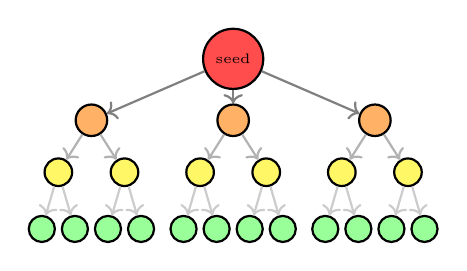
\begin{tikzpicture}[scale=0.6]
    % Layer 0 (seed)
    \node[circle, draw, thick, fill=red!70, minimum size=0.5cm] (s) at (0, 0) {\tiny seed};

    % Layer 1 (3 neighbors)
    \foreach \i in {1,2,3} {
        \pgfmathsetmacro{\x}{(\i-2)*3}
        \node[circle, draw, thick, fill=orange!60, minimum size=0.4cm] (n1\i) at (\x, -1.3) {};
        \draw[->, thick, gray] (s) -- (n1\i);
    }

    % Layer 2 (6 neighbors - 2 per L1 node)
    \foreach \i in {1,2,3} {
        \foreach \j in {1,2} {
            \pgfmathsetmacro{\x}{(\i-2)*3 + (\j-1.5)*1.4}
            \node[circle, draw, thick, fill=yellow!60, minimum size=0.35cm] (n2\i\j) at (\x, -2.4) {};
            \draw[->, thick, gray!60] (n1\i) -- (n2\i\j);
        }
    }

    % Layer 3 (12 neighbors - 2 per L2 node)
    \foreach \i in {1,2,3} {
        \foreach \j in {1,2} {
            \foreach \k in {1,2} {
                \pgfmathsetmacro{\x}{(\i-2)*3 + (\j-1.5)*1.4 + (\k-1.5)*0.7}
                \node[circle, draw, thick, fill=green!40, minimum size=0.25cm] (n3\i\j\k) at (\x, -3.6) {};
                \draw[->, thick, gray!40] (n2\i\j) -- (n3\i\j\k);
            }
        }
    }
\end{tikzpicture}
\caption{K-hop neighborhood expansion visualization with simplified fanout [3, 2, 2]. Starting from a single seed node, each layer multiplies the node count by the fanout value, demonstrating the exponential growth pattern inherent in neighbor sampling.}
\label{fig:neighbor-expansion-tree}
\end{figure}
\vspace{-0.5cm}
\begin{figure}[H]
\centering
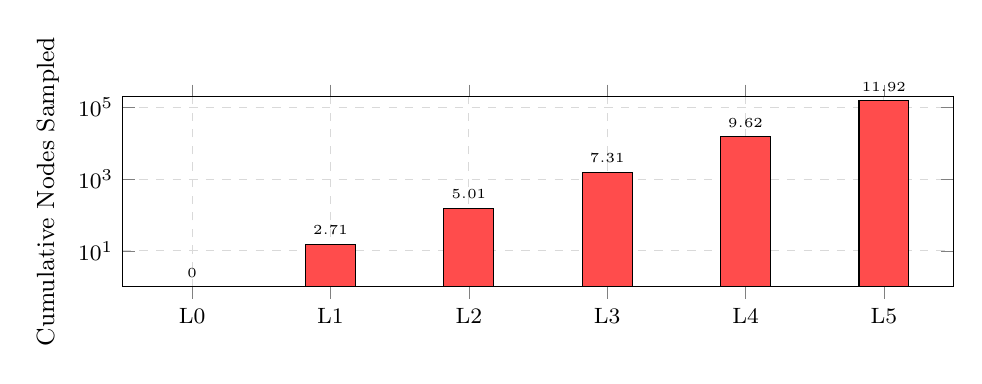
\begin{tikzpicture}
    \begin{axis}[
        ybar,
        symbolic x coords={L0, L1, L2, L3, L4, L5},
        xtick=data,
        ylabel={Cumulative Nodes Sampled},
        ymode=log,
        log origin=infty,
        width=\columnwidth,
        height=4cm,
        bar width=18pt,
        ymin=1,
        ymax=200000,
        ylabel style={font=\small},
        xlabel style={font=\small},
        tick label style={font=\footnotesize},
        grid=major,
        grid style={dashed, gray!30},
        nodes near coords,
        every node near coord/.append style={font=\tiny, rotate=0, anchor=south}
    ]
    \addplot[fill=red!70] coordinates {
        (L0, 1)
        (L1, 15)
        (L2, 150)
        (L3, 1500)
        (L4, 15000)
        (L5, 150000)
    };
    \end{axis}
\end{tikzpicture}
\caption{Memory explosion with real fanout configuration [15, 10, 10, 10, 10]. Each layer multiplies the sampled nodes, reaching 150,000 neighbors per seed node at layer 5. Combined across 128 seed nodes per batch, this yields 19.2M nodes consuming 30--40 GB of GPU memory. Note that the y-axis is logarithmic.}
\label{fig:neighbor-explosion}
\end{figure}

\subsection{Infrastructure and Software}
\label{subsec:infrastructure}

We use \textbf{PyTorch 2.1.2} (CUDA 12.1, cuDNN 8) with \textbf{PyTorch Geometric} for neighbor sampling (\texttt{NeighborLoader}) and GraphSAGE layers (\texttt{SAGEConv}). The pipeline is containerized via \textbf{Apptainer/Singularity} for reproducibility, bundling PyG, OGB, and compiled CUDA extensions.

\subsection{Distributed Training}
\label{subsec:ddp}

To overcome single-GPU memory limits, we use \textbf{PyTorch DDP} (Distributed Data Parallel) for multi-GPU training.

\paragraph{Why DDP and Not DeepSpeed?} The choice of DDP over more sophisticated frameworks like DeepSpeed is deliberate and based on our specific bottleneck analysis:
\begin{itemize}
    \item \textbf{Model size is tiny:} Our GraphSAGE model has only ${\sim}400$K parameters (${\sim}8$ MB), fitting comfortably in GPU memory. No model parallelism, tensor parallelism, or pipeline parallelism is needed.
    \item \textbf{Memory bottleneck is data, not parameters:} The memory pressure comes from sampled subgraphs (30--40 GB per batch), not model weights. DeepSpeed's Zero Redundancy Optimizer (ZeRO) optimizes parameter storage - irrelevant when parameters are negligible.
    \item \textbf{Data parallelism is sufficient:} The problem requires distributing \textit{data} (batches) across GPUs, not \textit{model} partitioning. DDP's simple data-parallel strategy is exactly what we need.
    \item \textbf{Simplicity and maintainability:} DDP requires minimal code changes and integrates seamlessly with PyTorch. DeepSpeed adds complexity (configuration files, custom optimizers) without tangible benefits for our use case.
\end{itemize}

In summary: \textbf{DeepSpeed solves the wrong problem}. Our bottleneck is subgraph storage, not model size. DDP's straightforward data parallelism is the optimal solution.

\paragraph{DDP Training Process.} The distributed training workflow consists of four key steps:
\begin{enumerate}
    \item \textbf{Process Initialization:} SLURM launches independent ranks per GPU (one process per GPU), each with its own Python interpreter and CUDA context. Processes communicate via the \textbf{NCCL} backend for GPU-to-GPU communication.
    \item \textbf{Data Partitioning:} The training set is split across ranks with no overlap. Each rank maintains an independent \newline \texttt{NeighborLoader} for k-hop sampling, with 4--8 worker processes prefetching batches per GPU.
    \item \textbf{Forward + Backward (Parallel):} Each GPU independently processes its batch, computes loss, and backpropagates gradients.
    \item \textbf{Gradient Synchronization:} DDP performs an all-reduce operation to average gradients across all GPUs, ensuring synchronized parameter updates via the optimizer step.
\end{enumerate}

\begin{figure}[H]
\centering
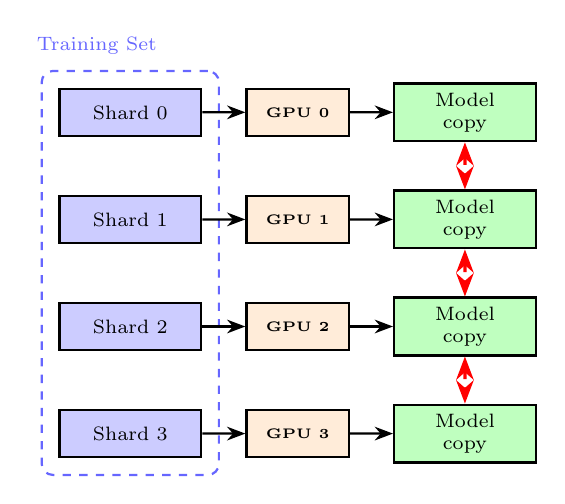
\begin{tikzpicture}[
    scale=0.85,
    boxstyle/.style={rectangle, draw, thick, minimum height=0.6cm, align=center},
    databox/.style={boxstyle, fill=blue!20, minimum width=1.8cm, font=\scriptsize},
    modelbox/.style={boxstyle, fill=green!25, minimum width=1.8cm, font=\scriptsize},
    gpubox/.style={boxstyle, fill=orange!15, minimum width=1.3cm, font=\tiny},
    arrow/.style={->, >=Stealth, thick},
    redarrow/.style={<->, >=Stealth, very thick, red, dashed}
]

% Data shards (left-center column)
\node[databox] (d0) at (-2.5, 3.2) {Shard 0};
\node[databox] (d1) at (-2.5, 1.6) {Shard 1};
\node[databox] (d2) at (-2.5, 0) {Shard 2};
\node[databox] (d3) at (-2.5, -1.6) {Shard 3};

% Box around all shards
\node[draw, thick, blue!60, dashed, rounded corners=4pt, inner sep=6pt, fit=(d0)(d3)] (shardbox) {};
\node[font=\scriptsize, blue!60, align=left] at (-3, 4.2) {Training Set};

% GPU labels (center)
\node[gpubox] (g0) at (0, 3.2) {\textbf{GPU 0}};
\node[gpubox] (g1) at (0, 1.6) {\textbf{GPU 1}};
\node[gpubox] (g2) at (0, 0) {\textbf{GPU 2}};
\node[gpubox] (g3) at (0, -1.6) {\textbf{GPU 3}};

% Model replicas (right-center column)
\node[modelbox] (m0) at (2.5, 3.2) {Model\\copy};
\node[modelbox] (m1) at (2.5, 1.6) {Model\\copy};
\node[modelbox] (m2) at (2.5, 0) {Model\\copy};
\node[modelbox] (m3) at (2.5, -1.6) {Model\\copy};

% Arrows connecting data -> GPU -> model
\foreach \i in {0,1,2,3} {
    \draw[arrow] (d\i) -- (g\i);
    \draw[arrow] (g\i) -- (m\i);
}

% Gradient sync arrows
\draw[redarrow] (m0) -- (m1);
\draw[redarrow] (m1) -- (m2);
\draw[redarrow] (m2) -- (m3);

\end{tikzpicture}
\caption{DDP architecture: data partitioned across GPUs, full model replicated per rank. Gradients synchronized via NCCL all-reduce after each batch. This data-parallel strategy is optimal when model size is small but data volume is large.}
\label{fig:ddp-architecture}
\end{figure}

Figure~\ref{fig:system-architecture} illustrates the complete system architecture, showing how SLURM orchestrates containerized training across multiple GPUs with partitioned data and NCCL-based gradient synchronization.

\begin{figure}[H]
\centering
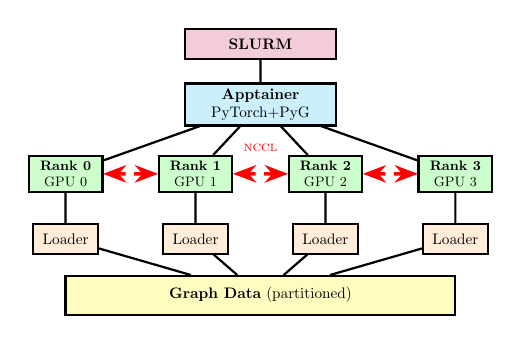
\begin{tikzpicture}[scale=0.55, every node/.style={transform shape}]

% Styles
\tikzset{
    boxstyle/.style={rectangle, draw, thick, minimum height=0.7cm, align=center},
    gpu/.style={boxstyle, fill=green!20, minimum width=1.7cm, font=\small},
    loader/.style={boxstyle, fill=orange!15, minimum width=1.5cm},
    graphbox/.style={boxstyle, fill=yellow!25, minimum width=9cm, minimum height=0.9cm},
    arrow/.style={-, >=Stealth, thick},
    redarrow/.style={<->, >=Stealth, very thick, red, dashed}
}

% Top layers
\node[boxstyle, fill=purple!20, minimum width=3.5cm] (slurm) at (0, 5.2) {\textbf{SLURM}};
\node[boxstyle, fill=cyan!20, minimum width=3.5cm] (container) at (0, 3.8) {\textbf{Apptainer}\\PyTorch+PyG};

% GPU ranks
\node[gpu] (r0) at (-4.5, 2.2) {\textbf{Rank 0}\\GPU 0};
\node[gpu] (r1) at (-1.5, 2.2) {\textbf{Rank 1}\\GPU 1};
\node[gpu] (r2) at (1.5, 2.2) {\textbf{Rank 2}\\GPU 2};
\node[gpu] (r3) at (4.5, 2.2) {\textbf{Rank 3}\\GPU 3};

% NCCL
\draw[redarrow] (r0) -- (r1);
\draw[redarrow] (r1) -- (r2);
\draw[redarrow] (r2) -- (r3);

% NCCL label
\node[font=\scriptsize, red] at (0, 2.8) {NCCL};

% Loaders
\node[loader] (l0) at (-4.5, 0.7) {Loader};
\node[loader] (l1) at (-1.5, 0.7) {Loader};
\node[loader] (l2) at (1.5, 0.7) {Loader};
\node[loader] (l3) at (4.5, 0.7) {Loader};

% Graph data
\node[graphbox] (gdata) at (0, -0.6) {\textbf{Graph Data} (partitioned)};

% Arrows
\draw[arrow] (slurm) -- (container);
\foreach \r in {r0,r1,r2,r3} {
    \draw[arrow] (container) -- (\r);
}
\foreach \i in {0,1,2,3} {
    \draw[arrow] (r\i) -- (l\i);
    \draw[arrow] (gdata) -- (l\i);
}

\end{tikzpicture}
\caption{System architecture for distributed GraphSAGE training. SLURM launches 4 containerized processes (one per GPU), each running an independent rank with its own NeighborLoader sampling from partitioned graph data. Gradients are synchronized across ranks via NCCL all-reduce.}
\label{fig:system-architecture}
\end{figure}

\subsection{Model Architecture}
\label{subsec:architecture}

Our GraphSAGE model consists of 5 layers, each using the \textbf{SAGEConv} layer with mean aggregation, followed by \textbf{LayerNorm}, \textbf{ReLU} activation, and \textbf{Dropout} (rate 0.5). The final layer is followed by a linear classifier for the 47-class prediction task. The architecture follows: 100-dimensional input (ogbn-products node features) $\to$ 256-dimensional hidden representations $\to$ 47-dimensional output (class logits). The model contains approximately 400K parameters, totaling ${\sim}8$ MB in memory.

%=======================================================================
\section{Hyperparameters}
\label{sec:hyperparameters}
%=======================================================================

\subsection{Hyperparameter Tuning Methodology}
\label{subsec:tuning-methodology}

To systematically explore the hyperparameter space and identify optimal configurations for large-scale GraphSAGE training, we developed a scalable and reproducible benchmarking pipeline. The goal is to enable \textbf{systematic, parallel hyperparameter optimization} on HPC infrastructure while maintaining complete reproducibility.

\paragraph{Benchmark Pipeline Architecture.}
Our pipeline follows a CSV-driven workflow:
\begin{enumerate}
    \item \textbf{Configuration Encoding:} Hyperparameter combinations are encoded in a \texttt{hyperparams.csv} file, with each row representing one training configuration.
    \item \textbf{SLURM Job Arrays:} Job arrays execute multiple training runs in parallel across the cluster. Each array task reads a specific configuration row by index (\texttt{\$SLURM\_ARRAY\_TASK\_ID}).
    \item \textbf{Containerized Training:} All experiments run within Apptainer containers (based on \newline \texttt{pytorch/pytorch:2.1.2-cuda12.1-cudnn8-runtime}) to ensure identical environments across cluster nodes and eliminate dependency variability.
    \item \textbf{DDP Training Execution:} Each job launches distributed training across 4 GPUs using PyTorch DDP, with training progress and final metrics logged.
    \item \textbf{Result Aggregation:} Training jobs write results (accuracy, loss, time, memory) to a shared \texttt{results.csv} file with file locking to prevent concurrent write conflicts.
    \item \textbf{Automated Analysis:} Python plotting scripts (\texttt{plotter.py}) aggregate results, compute statistics, and generate comparative visualizations.
\end{enumerate}

This architecture enables efficient parallel exploration of multiple hyperparameter configurations while maintaining scientific rigor through containerization and automated logging.

\subsection{Hyperparameter Space}
\label{subsec:hyperparameter-space}

We explored three primary dimensions affecting training performance and model quality: \textbf{mini-batch sampling} (batch size and gradient accumulation), \textbf{neighbor sampling} (fanout strategies), and \textbf{GPU scaling} (distributed training). Table~\ref{tab:hyperparameters} summarizes the tested parameters and their ranges, as well as fixed architectural and training hyperparameters.

\begin{table}[!htbp]
\centering
\caption{Hyperparameter configurations tested and fixed values}
\label{tab:hyperparameters}
\small
\begin{tabular}{@{} p{0.45\columnwidth} p{0.45\columnwidth} @{}}
\toprule
\multicolumn{2}{c}{\textbf{Tested Parameters}} \\
\midrule
Batch size & 16, 32, 64, 128, 160, 192, 256, 512 \\
Gradient accumulation & 1, 2, 3, 4, 5 \\
Neighbor fanout & 16 configurations \\
GPU count & 1, 2, 4, 8 \\
\midrule
\multicolumn{2}{c}{\textbf{Fixed Parameters}} \\
\midrule
Layers & 5 \\
Hidden dimensions & 256 \\
Learning rate & 0.003 \\
Epochs & 150 \\
Early stopping patience & 10 \\
Dropout rate & 0.5 \\
\bottomrule
\end{tabular}
\end{table}

\paragraph{Effective Batch Size.}
The effective batch size is computed as:
\[
\text{Effective Batch Size} = \text{batch\_size} \times \text{accum\_steps} \times \text{world\_size}
\]
where \texttt{world\_size} is the number of GPUs. For example, with batch size 128, accumulation steps 5, and 4 GPUs, the effective batch size is $128 \times 5 \times 4 = 2560$.

\subsection{Configurations Tested}
\label{subsec:configs-tested}

In total, we evaluated \textbf{36 hyperparameter configurations} organized into three benchmark categories:

\paragraph{Mini-Batch Sampling (16 configurations).} We tested combinations of batch size (16, 32, 64, 128, 160, 192, 256, 512) and gradient accumulation steps (1--5). The goal was to understand the trade-off between training time per epoch, peak GPU memory usage, and overall training efficiency. Batch sizes beyond 160 exceeded the 40 GB A100 memory limit and resulted in out-of-memory (OOM) errors.

\paragraph{Neighbor Sampling (16 configurations).} We explored diverse fanout strategies to balance accuracy, training time, and memory consumption. We tested the original baseline configuration ([15, 10, 10, 10, 10]), uniform samplers (e.g., [10,10,10,10,10]), increasing tapers (e.g., [3,5,10,15,20]), and layer ablation studies (e.g., [15,10,10,0,0]). 

\paragraph{GPU Scaling (4 configurations).} We evaluated distributed training scalability across 1, 2, 4 (single node), and 8 GPUs (2 nodes), with fixed batch size 128 and fanout [15,10,10,10,10]. The focus was on measuring speedup, parallel efficiency, and the impact of effective batch size on convergence.


%=======================================================================
\section{Results}\label{sec:results}
%=======================================================================

\subsection{Experimental Setup}

All benchmarking experiments were conducted on the MeluXina supercomputer using the Accelerator Module with 4x NVIDIA A100 GPUs (40GB each) per node. We evaluate three key dimensions: mini-batch sampling, neighbor sampling strategies, and GPU scaling.

\subsection{Mini-batch Sampling Benchmarking}

Mini-batch sampling controls the trade-off between training speed and GPU memory utilization. We varied batch size from 16 to 512 and gradient accumulation steps from 1 to 5, measuring training time per epoch and peak memory consumption. Figures~\ref{fig:batch-time} and \ref{fig:batch-memory} present the impact of batch size on these metrics.

\begin{figure}[H]
    \centering
    \includegraphics[width=\columnwidth]{../plots/time_per_epoch_vs_batch_size.png}
    \caption{Training time per epoch decreases with larger batch sizes due to better GPU utilization and reduced forward/backward pass overhead.}
    \label{fig:batch-time}
\end{figure}

\begin{figure}[H]
    \centering
    \includegraphics[width=\columnwidth]{../plots/peak_memory_vs_batch_size.png}
    \caption{Peak memory consumption scales linearly with batch size. Maximum reached batch size is 160, using ${\sim}32$ GB (with ${\sim}7.5$ GB system overhead).}
    \label{fig:batch-memory}
\end{figure}

\textbf{Key Findings:}
\begin{itemize}
    \item \textbf{Inverse relationship:} Larger batch sizes yield faster training per epoch due to better GPU utilization and amortized computational overhead.
    \item \textbf{Memory ceiling:} Batch sizes beyond 160 exceed the 40 GB A100 memory limit, resulting in OOM errors. The 160 batch size uses approximately 32 GB, leaving ${\sim}7.5$ GB for system overhead.
    \item \textbf{Optimal range:} Batch sizes 128--160 provide the best balance between memory efficiency and training speed.
\end{itemize}

\subsection{Neighbor Sampling Benchmarking}

Neighbor sampling strategy critically impacts both accuracy and computational cost. We tested 16 fanout configurations, including uniform strategies and layer ablation studies. The fanout determines the receptive field size and thus the amount of structural context available to the model, but also directly affects memory consumption through exponential neighborhood expansion. Figures~\ref{fig:neighbor-acc-time} and \ref{fig:neighbor-memory} illustrate the trade-offs between accuracy, training time, and memory consumption across various fanout configurations.

\begin{figure}[H]
    \centering
    \includegraphics[width=\columnwidth]{../plots/neighbor_efficiency_time_vs_accuracy.png}
    \caption{Accuracy-time trade-off. Upper-left region (high accuracy, low time) indicates efficient configurations. Moderate fanouts achieve the best balance.}
    \label{fig:neighbor-acc-time}
\end{figure}

\begin{figure}[H]
    \centering
    \includegraphics[width=\columnwidth]{../plots/neighbor_memory_vs_fanout.png}
    \caption{Memory consumption scales rapidly with total fanout ($F_{\text{total}} = \prod_{i=1}^{5} S_i$). High fanouts hit the 40 GB memory limit.}
    \label{fig:neighbor-memory}
\end{figure}

\textbf{Top Configurations (by Test Accuracy):}
\begin{center}
\small
\begin{tabular}{llll}
\toprule
\textbf{Rank} & \textbf{Fanout} & \textbf{Test Acc} & \textbf{Time (h)} \\
\midrule
1 & [15, 15, 15, 5, 5] & 0.8121 & 14.56 \\
2 & [15, 10, 10, 10, 0] & 0.8114 & 7.22 \\
\textbf{3} & \textbf{[15, 10, 10, 10, 10]} & \textbf{0.8096} & \textbf{19.53} \\
4 & [10, 10, 10, 10, 10] & 0.8088 & 16.46 \\
5 & [20, 15, 10, 5, 3] & 0.8055 & 11.60 \\
\bottomrule
\end{tabular}
\end{center}

\textbf{Key Findings:}
\begin{itemize}
    \item \textbf{Optimal efficiency:} Configuration [15,10,10,10,0] achieves near-baseline accuracy (81.14\% vs. 80.96\%) in only 7.22 hours, representing a \textbf{2.7$\times$ speedup} compared to the baseline [15,10,10,10,10]. This suggests that the model can be reduced to a 4-layer aggregation without significant accuracy loss.
    \item \textbf{Moderate fanouts dominate:} The upper-left region of the accuracy-time plot is populated by moderate fanout configurations. Very high fanouts provide no proportional accuracy gains and incur excessive memory and time costs.
    \item \textbf{Aggressive sampling hurts:} Extremely low fanouts (e.g., [5,5,5,5,5]) or single-layer strategies (e.g., [50,0,0,0,0]) either underperform or exhibit training instability.
\end{itemize}

\subsection{GPU Scaling Benchmarking}

Distributed training via PyTorch DDP enables efficient multi-GPU utilization. We evaluated scaling across 1, 2, 4 (single node), and 8 GPUs (2 nodes) with fixed hyperparameters (batch size 128, fanout [15,10,10,10,10]) to isolate the effect of parallelization. Training was limited to 10 epochs for faster benchmarking. Figures~\ref{fig:scaling-time} and \ref{fig:scaling-loss} show training time per epoch and training loss convergence across GPU counts.

\begin{figure}[H]
    \centering
    \includegraphics[width=\columnwidth]{../plots/scaling_time_per_epoch.png}
    \caption{Strong scaling demonstrates near-linear speedup up to 4 GPUs (93\% efficiency). Inter-node scaling to 8 GPUs achieves 89\% efficiency with modest degradation due to inter-node communication overhead.}
    \label{fig:scaling-time}
\end{figure}

\begin{figure}[htbp]
    \centering
    \includegraphics[width=\columnwidth]{../plots/scaling_train_loss.png}
    \caption{Training loss increases with GPU count due to larger effective batch sizes (512 for 4 GPUs, 1024 for 8 GPUs), resulting in reduced gradient noise.}
    \label{fig:scaling-loss}
\end{figure}

\textbf{Key Findings:}
\begin{itemize}
    \item \textbf{Strong intra-node scaling:} 1$\to$2 GPUs achieves 1.93$\times$ speedup (96.5\% efficiency); 1$\to$4 GPUs achieves 3.73$\times$ speedup (93\% efficiency). This demonstrates that PCIe/NVLink bandwidth is sufficient for gradient synchronization within a single node.
    \item \textbf{Acceptable inter-node scaling:} 1$\to$8 GPUs achieves 7.1$\times$ speedup (89\% efficiency). The 4\% efficiency drop relative to intra-node scaling is attributable to NCCL all-reduce communication over multi nodes, which introduces latency for gradient synchronization across nodes.
    \item \textbf{Loss-speed trade-off:} Larger effective batch sizes (batch\_size $\times$ world\_size = 512 for 4 GPUs, 1024 for 8 GPUs) lead to higher training loss due to reduced gradient noise. However, test accuracy remains competitive, justifying the 7$\times$ wall-clock speedup for distributed training.
\end{itemize}

%=======================================================================
\section{Discussion}
\label{sec:discussion}
%=======================================================================

\subsection{Bottlenecks Discovered}

\paragraph{Memory Wall.} The primary bottleneck is not computation but \textbf{memory}. Neighbor sampling causes exponential subgraph expansion: fanout [15,10,10,10,10] expands each seed node to approximately 150k neighbors. With batch size 128, this yields 19.2M nodes per batch, consuming 30--40 GB for subgraph storage and intermediate activations. In contrast, model parameters account for only $\sim$8 MB. This reveals that \textbf{sampled subgraphs dominate memory usage by 3--4 orders of magnitude over model parameters}, making memory - not compute - the critical resource constraint.

\paragraph{Inter-node Communication Overhead.} Gradient synchronization via NCCL over multiple nodes introduces communication overhead. Intra-node scaling (1$\to$4 GPUs) achieves 93\% efficiency via high-bandwidth NVLink/PCIe, while inter-node scaling (4$\to$8 GPUs) drops to 89\% efficiency. This 4\% degradation reflects the latency cost of all-reduce operations across network fabric, motivating careful consideration of when multi-node training is warranted.

\paragraph{Loss Convergence Trade-off.} Larger effective batch sizes (product of batch\_size, accum\_steps, and world\_size) lead to higher training loss. Effective batch sizes of 512 (4 GPUs) and 1024 (8 GPUs) reduce gradient noise, resulting in convergence to minima with higher loss. However, this increase in effective batch size can be mitigated by reducing the learning rate.

\subsection{What Worked Well}

\paragraph{DDP Implementation.} PyTorch's DistributedDataParallel seamlessly handles gradient synchronization with minimal code changes from the single-GPU baseline. The automatic all-reduce operations ensure consistent parameter updates across all ranks, abstracting away the complexity of distributed communication. This enabled us to scale from single-GPU to 8-GPU training with only minor modifications to the training loop.

\paragraph{Strong Intra-node Scaling.} The system scales nearly linearly up to 4 GPUs on a single node (3.73$\times$ speedup, 93\% efficiency), demonstrating that PCIe/NVLink provides sufficient bandwidth for gradient synchronization. This validates DDP as an effective approach for datasets that fit within the memory constraints of a single node but benefit from data parallelism.

\paragraph{Containerization.} Apptainer/Singularity ensured complete reproducibility across HPC environments by encapsulating the entire software stack (PyTorch 2.1.2, PyTorch Geometric, CUDA 12.1, cuDNN 8, and compiled CUDA extensions). This isolated complex dependencies, avoided version conflicts on shared clusters, and enabled seamless portability across different compute nodes.

\subsection{Key Trade-offs}

\begin{itemize}
    \item \textbf{Batch Size vs. Memory:} Batch 128--160 balances throughput and memory efficiency; further growth hits hard limits.
    \item \textbf{Receptive Field vs. Fanout:} Higher fanouts capture more context but cause exponential memory growth.
    \item \textbf{Speedup vs. Convergence:} 8 GPU training achieves 7x wall-clock speedup at the cost of slightly higher training loss.

\end{itemize}

\subsection{Lessons Learned}

\paragraph{Profile First, Optimize Second.} Early profiling revealed that memory - not computation - is the true bottleneck in large-scale GraphSAGE training. This insight guided our optimization efforts toward batch size tuning and fanout reduction rather than computational optimizations (e.g., kernel fusion, mixed-precision training). Without profiling, we might have pursued ineffective optimizations.

\paragraph{Trade-offs Are Inevitable.} Every optimization involves trade-offs, and there is no "free lunch." Larger batch sizes accelerate training but increase memory consumption and can hurt convergence. Higher fanouts improve accuracy but cause exponential memory growth. Distributed training provides speedup but introduces communication overhead and loss degradation. Effective system design requires balancing these competing objectives based on task priorities.

\paragraph{Reproducibility matters.} Containerization (Apptainer), fixed random seeds, and detailed logging are essential for rigorous scientific HPC work. Variability in system state (library versions, CUDA drivers, environment variables) can obscure true performance characteristics and make results non-reproducible. Our CSV-driven pipeline and containerized experiments ensure that all results can be independently verified.

\paragraph{Layer Ablation Insights.} The discovery that configuration [15,10,10,10,0] achieves better accuracy than the baseline (81.14\% vs. 80.96\%) with a 2.7$\times$ speedup demonstrates that the 5th layer contributes minimal additional context. This suggests that 4-hop neighborhood aggregation captures sufficient structural information for this dataset, and that \textbf{deeper is not always better} in GNN design.

%=======================================================================
\section{Conclusion}
\label{sec:conclusion}
%=======================================================================

This study demonstrates that GraphSAGE, when properly tuned and deployed on HPC infrastructure, scales effectively to large-scale node classification tasks. Key findings include: (1) batch sizes 128--160 offer optimal memory-speed trade-offs; (2) neighbor sampling strategy [15,10,10,10,0] achieves baseline accuracy with 2.7x speedup; (3) strong intra-node scaling validates multi-GPU deployment on a single node; (4) memory is the critical bottleneck, not computation.


%=======================================================================
\bibliographystyle{ACM-Reference-Format}
\bibliography{references}
%=======================================================================

\end{document}
